\chapter{lImporter}\label{chapter:proposal}
Este capítulo presenta la propuesta de \textit{lImporter}, un plugin para \textit{Obsidian} diseñado para automatizar la integración de nuevo conocimiento en una bóveda existente. El sistema recibe un conjunto de archivos y, guiado por instrucciones del usuario, genera y vincula nuevas notas de manera inteligente.

El problema fundamental que se aborda puede definirse formalmente. Se construye un Agente, $A$, que opera sobre una bóveda de \textit{Obsidian}. La función del agente es transformar la bóveda a un nuevo estado basándose en un conjunto de archivos de entrada y unas instrucciones específicas.

Sea $V$ el estado de la bóveda, definido como un conjunto de notas en formato \textit{Markdown}. Sea $F = \{f_1, f_2, \dots, f_n\}$ un conjunto de archivos de entrada y sea $I$ un conjunto de instrucciones en lenguaje natural que guían el proceso. La operación del agente se puede describir como una función:
\[ A(F, I, V) \rightarrow V' \]
donde $V'$ es la bóveda actualizada, que contiene nuevas notas, modificaciones a notas existentes y nuevos vínculos entre ellas, como resultado de la evaluación del agente. El conjunto de archivos de entrada $F$ puede estar compuesto por múltiples formatos. Para el reconocimiento de su contenido, se aprovecha la multimodalidad nativa de los modelos \textit{Gemini} \parencite{teamGeminiFamilyHighly2024}, que pueden procesar texto, imágenes y audio directamente. Esta arquitectura es modular: el componente de extracción de contenido puede ser reemplazado fácilmente por herramientas especializadas, como un sistema de reconocimiento óptico de caracteres (\textit{OCR}) para archivos \textit{PDF} o un servicio de \textit{speech-to-text} para audio.

\begin{figure}[h]
    \centering
    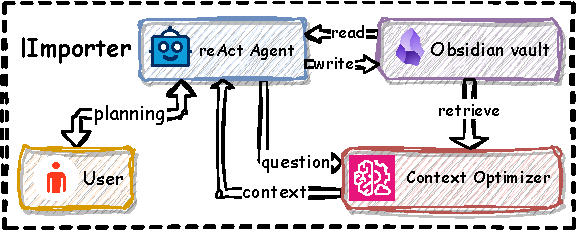
\includegraphics[width=0.85\textwidth]{figures/limporter.pdf}
    \caption{Esquema general del flujo de trabajo del agente en \textit{lImporter}.}
    \label{fig:importer_schema}
\end{figure}

Para la implementación de \textit{lImporter}, se propone un agente autónomo basado en el paradigma \textit{ReAct (Reasoning and Acting)}. Este agente está dotado de un conjunto de herramientas especializadas que le permiten interactuar directamente con la bóveda de \textit{Obsidian}, leyendo su estructura, obteniendo el contenido de las notas y escribiendo nueva información.

La explicación de la arquitectura se realizará de manera \textit{top-down}. Se comenzará describiendo el entorno y el funcionamiento general del agente, para luego profundizar en cada uno de sus componentes clave: el mecanismo de interacción con la bóveda y las estrategias para la obtención de contexto relevante.

\section{Descripción del entorno}
El entorno de trabajo para este proyecto es \textit{Obsidian}. A diferencia de otras herramientas basadas en la nube, el modelo de datos de \textit{Obsidian} es simple y robusto: una carpeta local en el sistema de archivos del usuario que contiene todos los datos. Las notas se almacenan como archivos de texto plano en formato \textit{Markdown} (`\textit{.md}`), y pueden organizarse en una jerarquía de carpetas tradicional. Este enfoque garantiza la portabilidad, la longevidad y el control total del usuario sobre su información.

Una de las características más distintivas de \textit{Obsidian} es su capacidad para visualizar las conexiones entre notas como un grafo de conocimiento. Cada nota es un nodo en el grafo, y los vínculos entre notas se representan como aristas. Esto permite al usuario descubrir relaciones emergentes y navegar por su conocimiento de una manera no lineal. El grafo de \textit{Obsidian} es un \textbf{grafo dirigido por fuerzas} (\textit{force-directed graph}), una simulación física donde los nodos se repelen entre sí, mientras que los enlaces actúan como resortes que los atraen. Este mecanismo provoca que los nodos con conexiones en común, incluso indirectas, se agrupen visualmente, revelando clústeres temáticos de forma intuitiva (ver Figura~\ref{fig:obsidian_force_graph_example}).

\begin{figure}[h]
    \centering
    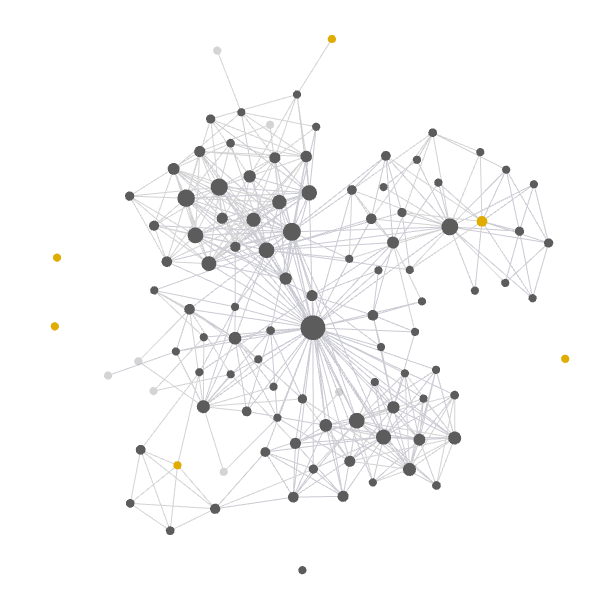
\includegraphics[width=0.66\textwidth]{figures/obsidian_kg_example.png}
    \caption{Ejemplo de la vista de grafo en \textit{Obsidian}, mostrando nodos y sus interconexiones.}
    \label{fig:obsidian_graph}
\end{figure}

La creación de vínculos es fundamental para construir el grafo. En \textit{Obsidian}, esto se logra mediante la sintaxis de \textit{wikilinks}, simplemente encerrando el nombre de otra nota entre dobles corchetes, por ejemplo, `[[Nota Destino]]`. Además de los vínculos simples, \textit{Obsidian} soporta la \textbf{transclusión}, que permite incrustar el contenido de una nota (o una sección de ella) dentro de otra usando la sintaxis `![[Nota a Incrustar]]`. En la estructura del grafo, tanto un vínculo simple `[[...]]` como una transclusión `![[...]]` crean una conexión directa y equivalente entre los nodos correspondientes, contribuyendo por igual a la dinámica de fuerzas. La transclusión, por tanto, enriquece el contenido de la nota sin alterar la naturaleza del vínculo en el grafo.

\begin{figure}[h!]
    \centering
    \begin{subfigure}[b]{0.48\textwidth}
        \centering
        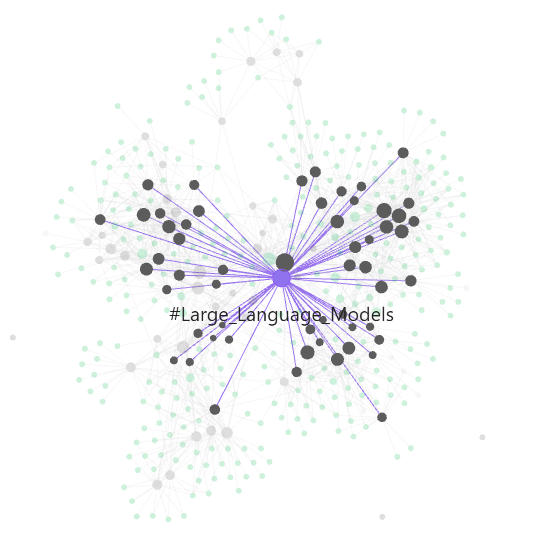
\includegraphics[width=\textwidth]{figures/LLM_tag_graph.png}
        % \caption{Vista del grafo centrada en la etiqueta \#Large Language Models.}
        \label{fig:llm_tag}
    \end{subfigure}
    \hfill
    \begin{subfigure}[b]{0.48\textwidth}
        \centering
        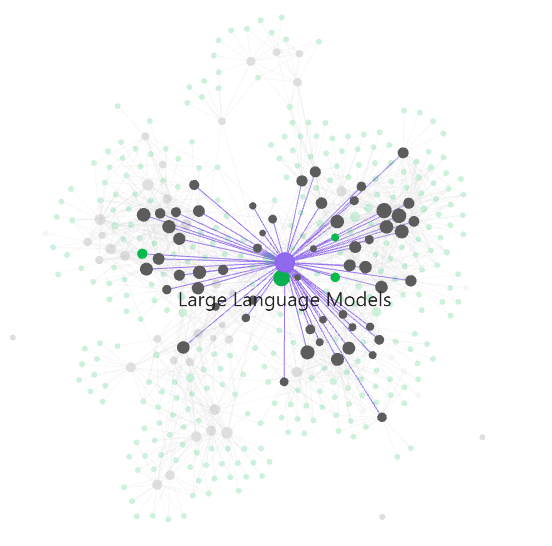
\includegraphics[width=\textwidth]{figures/LLM_note_graph.png}
        % \caption{Vista del grafo centrada en la nota Large Language Models.md.}
        \label{fig:llm_note}
    \end{subfigure}
    \caption{Comparación de la vecindad de la etiqueta \texttt{\#Large\_Language\_Models} y la nota \texttt{Large\_Language\_Models.md}.}
    \label{fig:obsidian_force_graph_example}
    \note{La proximidad visual entre el nodo de la etiqueta (izquierda) y el nodo de la nota (derecha) es un efecto directo del diseño basado en fuerzas. Al estar ambos conectados a un conjunto casi idéntico de notas, son atraídos hacia sus vecinos comunes, lo que resulta en su agrupación natural dentro del grafo.}
\end{figure}

\section{Agente \textit{reAct}}
En el núcleo del sistema se encuentra un agente basado en el \textit{framework ReAct} \parencite{yaoReActSynergizingReasoning2023}. Este paradigma permite a los modelos de lenguaje combinar el razonamiento (\textit{thought}) con la acción (\textit{action}). El agente opera en un ciclo donde, a partir de una tarea y una observación del entorno, razona sobre el siguiente paso a seguir, elige una herramienta de su repertorio, la ejecuta, y observa el resultado para informar su siguiente ciclo de razonamiento. En la práctica, este ciclo de \textit{Thought-Action-Observation} no es más que un bucle `while(true)` que se ejecuta hasta que se cumple una condición de parada. En la implementación, este bucle se acota a un número máximo de iteraciones para evitar ejecuciones infinitas. La sesión del agente finaliza de tres maneras: cuando el agente invoca una herramienta específica de finalización (e.g., \texttt{finish()}), cuando en su paso de razonamiento decide que la tarea está completa y no devuelve ninguna llamada a función, o cuando se alcanza el límite máximo de llamadas.

Siguiendo las mejores prácticas observadas en agentes avanzados como los utilizados para investigación o codificación (e.g. \textit{Deep Research}), se ha adoptado la estrategia \textit{Plan-and-Solve} \parencite{wangPlanandSolvePromptingImproving2023}. En lugar de actuar de forma impulsiva, el agente primero genera un plan detallado y paso a paso para resolver la tarea. El usuario tiene la opción de revisar, confirmar y dar retroalimentación sobre el plan generado antes de su ejecución. Este enfoque de \textit{human-in-the-loop} combina la eficiencia del planeamiento autónomo con la supervisión y el direccionamiento estratégico del usuario.

Para la implementación del agente se utiliza la familia de modelos \textit{Gemini} de \textit{Google}, debido a su multi-modalidad nativa, accesibilidad y, de manera crucial, su soporte nativo para \textit{function calling}, un mecanismo que se detallará a continuación.

\subsection{Interacción con la bóveda}
La capacidad del agente para leer y escribir archivos en la bóveda es posible gracias al uso de la \textit{API} de \textit{Obsidian}, orquestada a través de \textit{Function Calling}. Esta técnica puede ser entendida como un caso particular de \textit{style prompting} que emplea decodificación restringida (\textit{constrained decoding}) para forzar al modelo de lenguaje a generar una salida que se adhiere estrictamente a una gramática o formato predefinido \parencite{gengGrammarConstrainedDecodingStructured2024}.

En el caso de la \textit{API} de \textit{Gemini}, esta restricción obliga al modelo a producir una salida en formato \textit{JSON} que se corresponde con la firma de una de las funciones (herramientas) disponibles. Se aprovecha esta capacidad para mejorar la fiabilidad del agente. Por ejemplo, al definir los parámetros de una función, se puede utilizar el tipo de dato `\textit{ENUM}` para restringir las entradas a un conjunto de valores válidos (e.g., una lista de carpetas o archivos existentes), evitando así que el modelo intente operar sobre rutas inválidas o alucinadas.

\subsubsection{Lectura}
Para la lectura de información de la bóveda, el agente dispone de dos herramientas principales:
\begin{itemize}
    \item \texttt{tree(path)}: Esta función recibe la ruta a una carpeta raíz y devuelve una representación textual de la estructura de directorios y archivos contenida en ella, de forma análoga al comando \texttt{tree} de la línea de comandos. Esto permite al agente obtener una visión global de la organización de la bóveda.
    \item \texttt{read(path)}: Esta función recibe la ruta a un archivo \textit{Markdown} (`\textit{.md}`) existente y devuelve su contenido completo como texto.
\end{itemize}
 
\subsubsection{Escritura}
Un desafío común en los agentes que interactúan con sistemas de archivos es la tendencia del modelo a generar rutas de archivo incorrectas o con nombres similares pero no idénticos a los existentes. Para mitigar este problema, la capacidad de escritura se ha separado en dos funciones distintas:
\begin{itemize}
    \item \texttt{mkdir(path)}: Permite al agente crear un nuevo directorio en una ubicación específica de la bóveda, asegurando que la estructura de carpetas deseada exista antes de intentar escribir un archivo.
    \item \texttt{write(path, content)}: Crea un nuevo archivo o sobrescribe el contenido de uno existente. El parámetro \texttt{path} de esta función se beneficia directamente de la decodificación restringida, ya que se puede guiar al modelo para que elija entre rutas sugeridas o siga un formato válido, reduciendo drásticamente los errores.
\end{itemize}
 
\subsubsection{Obtencion de contexto}
Para que el agente pueda tomar decisiones informadas, como determinar dónde crear una nueva nota o con qué notas existentes vincularla, necesita un contexto relevante de la bóveda. Dado que el contenido total de la bóveda puede exceder fácilmente la ventana de contexto del modelo, se utiliza un enfoque de divide y vencerás.

Se propone una función que recibe un conjunto de archivos y un límite de tokens. Si el contenido combinado de los archivos excede el límite, el conjunto se divide recursivamente por la mitad hasta que los fragmentos resultantes son lo suficientemente pequeños. Una vez que un fragmento cabe en la ventana de contexto, un modelo de lenguaje se encarga de extraer la información relevante de él. La naturaleza de esta información relevante se define por un nivel de \textbf{granularidad} especificado por el usuario (en \cite{chenDenseRetrievalWhat2024} se analiza la optimalidad de selección de diferentes casos de estos).

Esta idea está inspirada en la técnica propuesta en \cite{shenQwenLongCPRS$infty$LLMsDynamic2025}. De manera similar, se proponen tres niveles de granularidad:
\begin{itemize}
    \item \textbf{Paragraph}: Ideal para obtener resúmenes y el sentido general de un documento.
    \item \textbf{Sentence}: Extremadamente útil para identificar afirmaciones específicas y recuperar relaciones entre conceptos.
    \item \textbf{Keyword}: Perfecto para la extracción de entidades nombradas y conceptos clave.
\end{itemize}

% Pseudocódigo del proceso de obtención de contexto:
\begin{figure}[h]
    \centering
    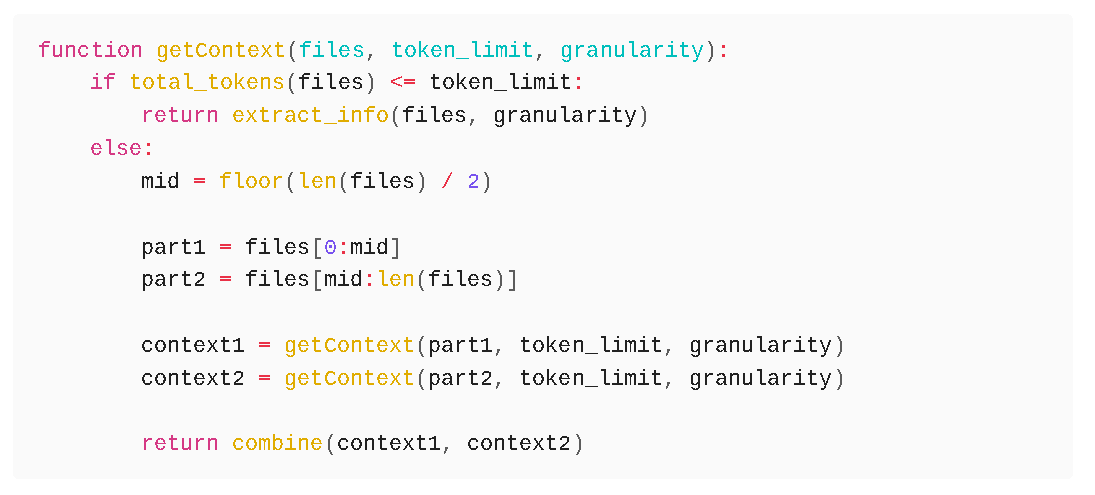
\includegraphics[width=1.0\textwidth]{figures/getContext.pdf}
    % \begin{verbatim}
    % function getContext(files, token_limit, granularity):
    %     if total_tokens(files) <= token_limit:
    %         return extract_info(files, granularity)
    %     else:
    %         mid = floor(len(files) / 2)
    %         part1 = files[0:mid]
    %         part2 = files[mid:len(files)]
            
    %         context1 = getContext(part1, token_limit, granularity)
    %         context2 = getContext(part2, token_limit, granularity)
            
    %         return combine(context1, context2)
    % \end{verbatim}
    \caption{Pseudocódigo del proceso de obtención de contexto.}
    \label{fig:alg_cprs}
\end{figure}


\subsection{Sobre la versatibilidad del sistema}
Un objetivo clave de \textit{lImporter} es su versatilidad para integrarse en diversos flujos de trabajo. El agente debe ser útil tanto para un usuario que desea construir una base de conocimiento densamente interconectada, generando múltiples relaciones y resúmenes, como para otro que simplemente quiere archivar un nuevo concepto de forma aislada, sin crear ningún vínculo.

La arquitectura basada en un agente \textit{ReAct} y el sistema de obtención de contexto granular sustentan esta flexibilidad. El agente puede recibir instrucciones para ser exhaustivo en la búsqueda de conexiones o, por el contrario, para limitarse a crear una nota y guardarla en una carpeta específica. Un ejemplo claro de esta flexibilidad es el proceso de selección de la ubicación para las nuevas notas. El sistema no prefija una carpeta de destino. En su lugar, el agente decide la ruta óptima en tiempo de ejecución basándose en una combinación de factores: las instrucciones iniciales del usuario, y las directrices que puede encontrar dentro del contenido de los propios archivos de entrada. Se le puede instruir, por ejemplo, para que lea un archivo \texttt{\_index.md} que guíe la organización de un subdirectorio. Esta libertad permite al usuario implementar tanto estructuras rígidas como flujos de trabajo donde las notas se crean de manera dispersa y emergente. Para garantizar la integridad de la bóveda, aunque el agente puede explorar cualquier ruta desde la raíz para tomar su decisión, al momento de ejecutar la acción de escritura, los parámetros de la función se validan. Como se mencionó, se le presenta al modelo una lista de las carpetas existentes en un formato `\textit{ENUM}`, lo que restringe su elección a una ruta válida y previene errores.

Sin embargo, esta versatilidad conlleva un incremento en la labor manual de configuración inicial, ya que el comportamiento del agente se define en gran medida a través de un archivo de instrucciones proporcionado por el usuario.

\begin{figure}[h!]
    \centering
    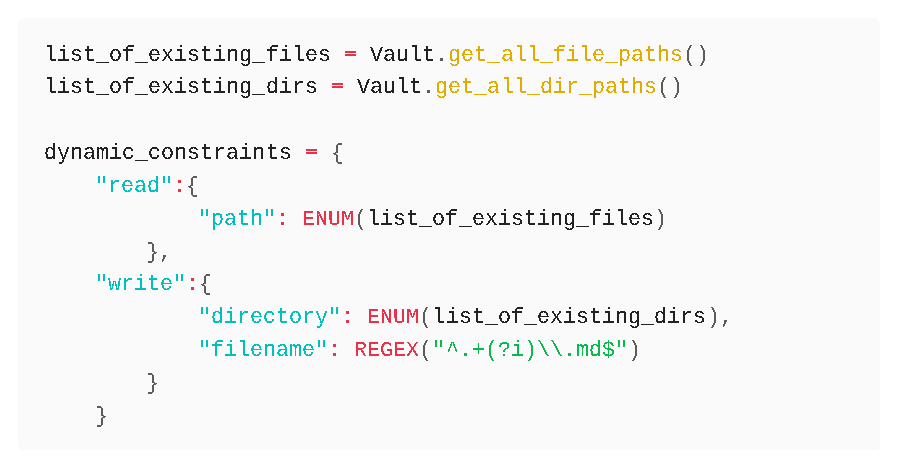
\includegraphics[width=\textwidth]{figures/pseudoConstrnt.pdf}
    \caption{Flujo de decodificación restringida para la interacción con el sistema de archivos. El agente expresa una intención, el sistema traduce las rutas válidas en restricciones y la API del modelo genera una llamada a herramienta que está garantizada para ser ejecutable.}
    \label{fig:constrained_decoding}
    \note{Es importante aclarar que, al momento de la implementación, la API de \textit{Gemini} no soporta de forma nativa la validación de parámetros mediante expresiones regulares (\textit{regex}) en la definición de herramientas. Sin embargo, en la práctica, el modelo rara vez comete errores en la generación de nombres de archivo con el formato adecuado (por ejemplo, omitiendo la extensión \texttt{.md}). En cualquier caso, esta validación se puede implementar de forma trivial como un paso de post-procesamiento: el sistema recibe la llamada a la función generada por el modelo y verifica la validez del nombre del archivo antes de ejecutar la acción de escritura en el disco.}
\end{figure}

\begin{figure}[h!]
    \centering
    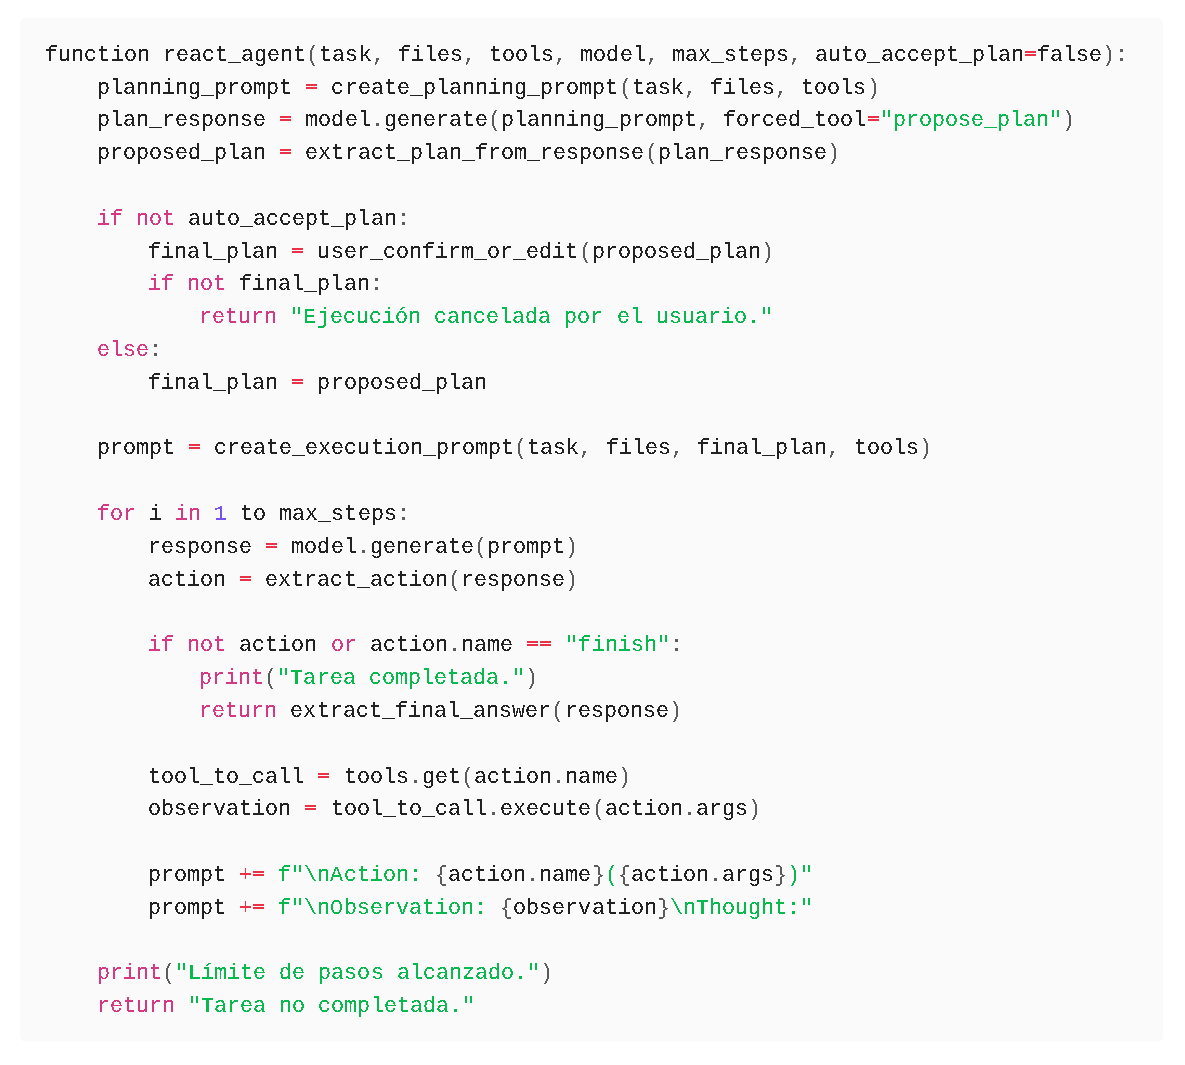
\includegraphics[width=1.0\textwidth]{figures/pseudoReAct.pdf}
% \begin{verbatim}
%     function react_agent(task, files, tools, model, max_steps, auto_accept_plan=false):
%     // --- Fase 1: Planificación (Estrategia Plan-and-Solve) ---
%     // Se crea un prompt inicial para que el agente genere un plan.
%     // Se 'fuerza' al modelo a usar una herramienta 'propose_plan' para asegurar
%     // que su primera acción sea la creación de un plan estructurado.
%     planning_prompt = create_planning_prompt(task, files, tools)
%     plan_response = model.generate(planning_prompt, forced_tool="propose_plan")
%     proposed_plan = extract_plan_from_response(plan_response)

%     // --- Fase de Intervención Humana (Human-in-the-loop) ---
%     // El plan puede ser auto-aceptado o requerir confirmación del usuario.
%     if not auto_accept_plan:
%         final_plan = user_confirm_or_edit(proposed_plan)
%         if not final_plan:
%             return "Ejecución cancelada por el usuario."
%     else:
%         final_plan = proposed_plan
    
%     // --- Fase 2: Ejecución del Plan con el ciclo ReAct ---
%     // El plan aprobado se añade al historial para guiar los siguientes pasos del agente.
%     prompt = create_execution_prompt(task, files, final_plan, tools)

%     for i in 1 to max_steps:
%     // 1. Reason (Thought) & 2. Action
%         response = model.generate(prompt)
%         action = extract_action(response) // e.g., {name: "tool_name", args: {...}}

%         if not action or action.name == "finish":
%             print("Tarea completada.")
%             return extract_final_answer(response)

%         // 3. Observation
%         tool_to_call = tools.get(action.name)
%         observation = tool_to_call.execute(action.args)

%         // Se actualiza el prompt con el resultado de la acción para el siguiente ciclo.
%         prompt += f"\nAction: {action.name}({action.args})"
%         prompt += f"\nObservation: {observation}\nThought:"

%     print("Límite de pasos alcanzado.")
%     return "Tarea no completada."
% \end{verbatim}
    \caption{Pseudocódigo del ciclo de ejecución del agente \textit{ReAct}.}
    \label{fig:react_agent_pseudocode}
    \note{Cabe señalar que el pseudocódigo presentado es una representación conceptual y simplificada del ciclo \textit{ReAct}. En la práctica, se usa una implementación más sofisticada del paradigma. En lugar de gestionar el flujo mediante la concatenación manual de prefijos de texto (como \texttt{Thought:} u \texttt{Observation:}), una técnica común en tareas de predicción de texto simple, la interacción se gestiona de forma más integrada a través de la API del modelo. Esto implica mantener un historial de conversación estructurado, donde cada llamada a una herramienta y su correspondiente resultado (la observación) se añaden como mensajes distintos en el diálogo, aprovechando directamente las capacidades nativas de \textit{function calling}.}
\end{figure}